\chapter{SYSTEM DESIGN AND IMPLEMENTATION}
\label{chap:caseFarming}

This chapter describes the implementation of the system which consists of two subsystems: A social media website and an analysis server. In \textit{Requirement analysis and System overview} subsection, everything is briefly described as a whole. In three last sections, structure and details of two subsystems and the database are defined more comprehensively.

\section{Requirement analysis and system overview}
\subsection{Requirement analysis}

\subsection{System overview}
Figure \ref{chap3:system_overview_basic} shows a concise overview of how the system operates. Users interact with the website through front-end. The input of users can come in the form of images, videos or label contribution. Back-end receives input and stores in the database. Concurrently, inputs are sent to analysis server . Outputs from analysis server are sent back to back-end and then stored in database. The back-end is also responsible for obtaining appropriate contents from the database to display to users through front-end.

\begin{center}
    \begin{figure}[H]
    \centering
    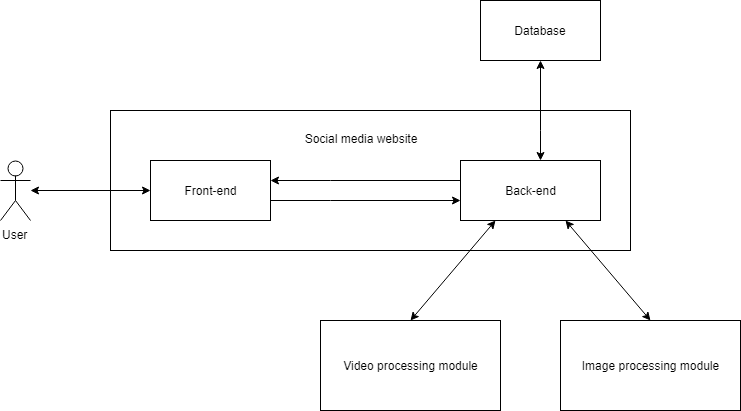
\includegraphics[width=1\columnwidth]{images/chap3/system_overview_basic.png}
    \caption{An overview of the system}
    \label{chap3:system_overview_basic}
    \end{figure}
\end{center}

\section{Social media website}

\subsection{Database}
The project database divides into two different parts: \textbf{Cloud storage} and a \textbf{NoSQL database}. The primary target is to reduce website loading time. Let take an example, if files are stored directly on the crowd-sourcing server. When many users request a file simultaneously, the server with limited bandwidth will cause delay. “53\% of mobile site visitors leave a page that takes longer than three seconds to load” – \href{https://think.storage.googleapis.com/docs/mobile-page-speed-new-industry-benchmarks.pdf}{Google}. If these files stored on cloud storage, the client will be served by the cloud storage provider, which has higher availability.
\section{Analysis server}
The project requires two systems for analysis: A face recognition system and a video classifier system. The facial recognition system takes pictures of human faces as input and returns their identification. The video classifier system analyzes videos to find out actions in them. The remaining of this section describes in detail about the two analysis system.
\subsection{Face recognition module}
\subsection{Video classifier module}
Video classifying is not a new task in the field of Deep learning.
	
\section{Technologies}
\subsection{Node.js and npm}
Node.js (Node) is a JavaScript runtime built on Chrome's V8 JavaScript engine (cite). Node supports executing JavaScript on server-side. Ryan Dahl was created Node.js in 2009. Node.js Foundation is in charge of the development of Node.js. After nine years since its release, the latest LTS version of Node.js is 10.14.2 (includes npm 6.4.1). “Node.js operates on a single thread, using non-blocking I/O calls, allowing it to support tens of thousands (cite) of concurrent connections held in the event loop.” Although JavaScript is single-threaded, thanks to the Event loop, Node.js can implement asynchronous I/O operations. The Event loop will transfer operations to the system kernel. “Since most modern kernels are multi-threaded, they can handle multiple operations executing in the background. When one of these operations completes, the kernel tells Node.js so that the appropriate callback may be added to the poll queue to executed eventually”. By utilizes non-blocking I/O, Node.js skips the waiting time for I/O calls, which is much higher than processing time.
\section{Implementation}